%\documentclass[handout]{beamer}
\documentclass{beamer}
 
\usetheme[numbering = fraction, progressbar = none, background = light, sectionpage = progressbar]{metropolis}
\usepackage{amsmath}
\usepackage{tabu}
\usepackage{graphicx}

\title{Econ 103 -- Statistics for Economists}
\subtitle{Chapter 4 and 5: Continuous Random Variables}
\author{Mallick Hossain}
\date{}
\institute{University of Pennsylvania}
\begin{document} 

%%%%%%%%%%%%%%%%%%%%%%%%%%%%%%%%%%%%%%%%
\begin{frame}
	\titlepage 
\end{frame} 

%%%%%%%%%%%%%%%%%%%%%%%%%%%%%%%%%%%%%%%%
\begin{frame}
\frametitle{Why Are Continuous RVs Important?}
\begin{itemize}[<+-|alert@+>]
	\item Continuous RVs will be the foundation upon which we will build the statistical portion of the course
	\item Normal, chi-squared, t-, and F-distributions are all continuous random variables
	\item By learning the discrete RVs, you have developed an intuition about random variables that will translate into intuition about continuous RVs. 
	\item This is a good chance to solidify your understanding of RVs. 
	\item If you have an intuitive understanding of continuous RVs (especially the normal distribution), the rest of the semester will seem easy.
\end{itemize}
\end{frame}

%%%%%%%%%%%%%%%%%%%%%%%%%%%%%%%%%%%%%%%%
\begin{frame}
\frametitle{Continuous RVs -- What Changes?}
	\begin{enumerate}
\item Probability Density Functions replace Probability Mass Functions (aka Probability Distributions)
\item Integrals Replace Sums
\end{enumerate}
\begin{alertblock}{Everything Else is Essentially Unchanged!}\end{alertblock}

\end{frame}

\section{Twister}
%%%%%%%%%%%%%%%%%%%%%%%%%%%%%%%%%%%%%%%%
\begin{frame}
\frametitle{What is the probability of ``Yellow?''}
\centering
	\includegraphics[scale = 0.6]{./images/twister}

\end{frame}

%%%%%%%%%%%%%%%%%%%%%%%%%%%%%%%%%%%%%%%
\begin{frame}
\frametitle{What is the probability of ``Right Hand Blue?'' }
\centering
	\includegraphics[scale = 0.6]{./images/twister}
\end{frame}

%%%%%%%%%%%%%%%%%%%%%%%%%%%%%%%%%%%%%%%
\begin{frame}
\frametitle{What is the probability that the spinner lands in any \emph{particular} place?}

\begin{center}
	\includegraphics[scale = 0.6]{./images/twister}
\end{center}
\end{frame}

%%%%%%%%%%%%%%%%%%%%%%%%%%%%%%%%%%%%%%%%
\begin{frame}
\frametitle{From Twister to Density -- Probability as \emph{Area}}

\centering
	\includegraphics[scale = 0.55]{./images/twister_density}
\end{frame}

\section{PDFs and CDFs for Continuous RVs}
%%%%%%%%%%%%%%%%%%%%%%%%%%%%%%%%%%%%%%%%
\begin{frame}
\frametitle{Continuous Random Variables}
For continuous RVs, probability will be the area of \emph{intervals} because \alert{individual points have zero probability.}
\end{frame}

%%%%%%%%%%%%%%%%%%%%%%%%%%%%%%%%%%%%%%%%
\begin{frame}
\frametitle{Probability Density Function (PDF)}
For a continuous random variable $X$, 
	$$P(a \leq X \leq b) = \int_a^b f(x) \; dx$$
where $f(x)$ is the \emph{probability density function} for $X$. 
\vspace{2em}

\begin{alertblock}{Extremely Important}
For any realization $x$, $P(X=x) = 0 \neq f(x)$!
\end{alertblock}
\end{frame}

%%%%%%%%%%%%%%%%%%%%%%%%%%%%%%%%%%%%%%%%
\begin{frame}
\frametitle{Properties of PDFs}
\begin{enumerate}
\item $\int_{-\infty}^\infty f(x) \; dx = 1$ 
\item $f(x) \geq 0$ for all $x$
\item $f(x)$ is \emph{not} a probability and can be greater than one!
\item $P(X\leq x_0) = F(x_0) = \int_{-\infty}^{x_0} f(x) \; dx $
\end{enumerate}
\end{frame}

\section{Expectation and Variance}
%%%%%%%%%%%%%%%%%%%%%%%%%%%%%%%%%%%%%%%%
\begin{frame}
\frametitle{Expectation of Continuous RVs}

\begin{itemize}[<+-|alert@+>]
	\item Recall that for discrete RVs, $E[X] = \sum_{i = 1}^n x_i p(x_i)$
	\item For continuous RVs, expected value is similar
	$$
	E[X] = \int_{-\infty}^\infty x f(x) dx
	$$
	\item The integral replaces the sum!
	\item The definition holds for functions of the RV as well
	$$
	E[g(X)] = \int_{-\infty}^\infty g(x) f(x) dx
	$$
\end{itemize}	
\end{frame}

%%%%%%%%%%%%%%%%%%%%%%%%%%%%%%%%%%%%%%%%
\begin{frame}
\frametitle{What about all those rules for expected value?}
\begin{itemize}
  \item The only difference between expectation for continuous versus discrete is how we do the \emph{calculation}.
  \item Sum for discrete; integral for continuous.
  \item All \emph{properties} of expected value \alert{continue to hold!}
  \item Includes linearity, shortcut for variance, etc.
\end{itemize}
\end{frame}

%%%%%%%%%%%%%%%%%%%%%%%%%%%%%%%%%%%%%%%%
\begin{frame}
\frametitle{Variance of Continuous RV}

\begin{itemize}[<+-|alert@+>]
	\item Recall that for discrete RVs, $Var[X] = E[(X - E[X])^2]$
	\item For continuous RVs, expected value is the same, just with the different formula for expectation
	\begin{align*}
	Var[X] &= E[(X - E[X])^2]
	\\
	&= \int_{-\infty}^\infty (x - \mu)^2 f(x) dx
	\end{align*}
	\item Shortcut formula still holds!
	$$
	Var(X) = E[X^2] - \left(E[X]\right)^2
	$$
\end{itemize}	
\end{frame}

%%%%%%%%%%%%%%%%%%%%%%%%%%%%%%%%%%%%%%%%
\begin{frame}
\frametitle{We're Won't Say More About These, But Just So You're Aware of Them...}

\begin{block}{Joint Density}
$ \displaystyle P(a\leq X \leq b \cap c\leq Y \leq d) = \int_c^d \int_a^b f(x,y) \; dxdy$
\end{block}
\begin{block}{Marginal Densities}
$f_X(x) = \int_{-\infty}^\infty f(x,y)\; dy$, $\;\;\;\;\;\;\; f_Y(y) = \int_{-\infty}^\infty f(x,y)\; dx$
\end{block}
\begin{block}{Independence in Terms of Joint and Marginal Densities}
$f_{XY}(x,y) = f_X(x)f_Y(y)$
\end{block}
\begin{block}{Conditional Density}
$f_{Y|X} = \frac{f_{XY}(x,y)}{f_X(x)}$
\end{block}

\end{frame}

\section{Uniform Random Variable}
%%%%%%%%%%%%%%%%%%%%%%%%%%%%%%%%%%%%%%%%
\begin{frame}
\frametitle{Simplest Possible Continuous RV: Uniform$(0,1)$}

\begin{block}{$X \sim \mbox{Uniform}(0,1)$}
A Uniform(0, 1) RV is equally likely to take on \emph{any value} in the range $[0,1]$ and never takes on a value outside this range.
\end{block}

\begin{block}{Uniform PDF}
$f(x) = 1$ for $0\leq x \leq 1$, zero elsewhere.
\end{block}

\end{frame}
%%%%%%%%%%%%%%%%%%%%%%%%%%%%%%%%%%%%%%%%


\begin{frame}
\frametitle{Uniform$(0,1)$ PDF}
\centering
	\includegraphics[scale = 0.5]{./images/uniform_density}

\end{frame}


%%%%%%%%%%%%%%%%%%%%%%%%%%%%%%%%%%%%%%%%
\begin{frame}
\frametitle{What is the area of the shaded region? }

\centering
	\includegraphics[scale = 0.5]{./images/uniform_density_shaded}

\end{frame}


%%%%%%%%%%%%%%%%%%%%%%%%%%%%%%%%%%%%%%%%

\begin{frame}
\frametitle{What is the area of the shaded region?}

\centering
	\includegraphics[scale = 0.4]{./images/uniform_density_shaded}
\begin{eqnarray*}
	\int_{-\infty}^{\infty} f(x) \; dx = \int_{0}^1 1 \; dx = \left. x \right|_0^1 = 1 - 0 = 1
\end{eqnarray*}
\end{frame}


%%%%%%%%%%%%%%%%%%%%%%%%%%%%%%%%%%%%%%%%



\begin{frame}
\frametitle{What is the area of the shaded region?}
\centering
	\includegraphics[scale = 0.5]{./images/uniform_density_cdf}

\end{frame}


%%%%%%%%%%%%%%%%%%%%%%%%%%%%%%%%%%%%%%%%

\begin{frame}
\frametitle{$F(0.4) = P(X\leq 0.4) = 0.4$}
\centering
	\includegraphics[scale = 0.5]{./images/uniform_density_cdf}

\end{frame}


%%%%%%%%%%%%%%%%%%%%%%%%%%%%%%%%%%%%%%%%


\begin{frame}
\frametitle{Relationship between PDF and CDF}

Integrate pdf $\rightarrow$ CDF
	$$F(x_0) = P(X\leq x_0) = \int_{-\infty}^{x_0} f(x)\; dx$$
Differentiate CDF $\rightarrow$ pdf
 	$$f(x) =\frac{d}{dx}F(x)$$
\alert{This is just the First Fundamental Theorem of Calculus.}
\end{frame}


%%%%%%%%%%%%%%%%%%%%%%%%%%%%%%%%%%%%%%%%
\begin{frame}
\frametitle{Example: Uniform$(0,1)$ RV}

Integrate the pdf, $f(x) = 1$, to get the CDF
\begin{eqnarray*}
	F(x_0) =\int_{-\infty}^{x_0} f(x)\; dx = \int_{0}^{x_0} 1\; dx =  \left. x \right|_0^{x_0} =  x_0 - 0 = x_0
\end{eqnarray*}

\vspace{1em}
$$ F(x_0) = \left\{ \begin{array}{c} 0, x_0 < 0\\ x_0, 0\leq x_0 \leq 1\\ 1, x_0 > 1   \end{array}\right.$$
\end{frame}


%%%%%%%%%%%%%%%%%%%%%%%%%%%%%%%%%%%%%%%%
\begin{frame}
\frametitle{Uniform$(0,1)$ CDF}
\centering
	\includegraphics[scale = 0.5]{./images/uniform_CDF}

\end{frame}


%%%%%%%%%%%%%%%%%%%%%%%%%%%%%%%%%%%%%%%%
\begin{frame}
\frametitle{Example: Uniform$(0,1)$ RV}
Differentiate the CDF, $F(x_0) = x_0$, to get the pdf
 \begin{eqnarray*}
	\frac{d}{dx}F(x) =  1 = f(x)
 \end{eqnarray*}
\end{frame}



%%%%%%%%%%%%%%%%%%%%%%%%%%%%%%%%%%%%%%%%
\begin{frame}
\frametitle{What is $P(0.4 \leq X \leq 0.8)$ if $X\sim \mbox{Uniform}(0,1)$? }
\centering
	\includegraphics[scale = 0.5]{./images/uniform_density_interval}


\end{frame}
%%%%%%%%%%%%%%%%%%%%%%%%%%%%%%%%%%%%%%%%
\begin{frame}
\frametitle{$F(0.8) = P(X \leq 0.8)$}

\centering
	\includegraphics[scale = 0.5]{./images/density_interval_cdf1}

\end{frame}


%%%%%%%%%%%%%%%%%%%%%%%%%%%%%%%%%%%%%%%%
\begin{frame}
\frametitle{$F(0.8) - F(0.4) = $ ?}
\centering
	\includegraphics[scale = 0.5]{./images/density_interval_cdf2}

\end{frame}


%%%%%%%%%%%%%%%%%%%%%%%%%%%%%%%%%%%%%%%%
\begin{frame}
\frametitle{$F(0.8) - F(0.4) = P(0.4 \leq X \leq 0.8) = 0.4$}
\centering
	\includegraphics[scale = 0.5]{./images/uniform_density_interval}


\end{frame}
%%%%%%%%%%%%%%%%%%%%%%%%%%%%%%%%%%%%%%%%
\begin{frame}
\frametitle{Key Idea: Probability of Interval for Continuous RV}

$$\boxed{P(a\leq X \leq b) = \int_a^b f(x) \; dx = F(b) - F(a)}$$

\vspace{2em}
\alert{This is just the Second Fundamental Theorem of Calculus.}
\end{frame}

%%%%%%%%%%%%%%%%%%%%%%%%%%%%%%%%%%%%%%%%
\begin{frame}
\frametitle{Example: Uniform(0,1) Random Variable }
\begin{eqnarray*}
	E[X] &=&  \int_{-\infty}^\infty x f(x) \; dx =\pause  \int_{0}^1 x \cdot 1 \; dx \\ \\
		&=&  \left.\frac{x^2}{2}\right|_0^1 = 1/2  - 0 = 1/2
\end{eqnarray*}
\end{frame}

%%%%%%%%%%%%%%%%%%%%%%%%%%%%%%%%%%%%%%%%

\begin{frame}
\frametitle{Example: Uniform(0,1) Random Variable }
	\begin{eqnarray*}
	E[X^2] &=& \int_{-\infty}^\infty x^2 f(x) \; dx \pause = \int_0^1 x^2 \cdot 1 \; dx\\ \\
		&=& \left. \frac{x^3}{3}\right|_0^1 = 1/3
	\end{eqnarray*}
\end{frame}


%%%%%%%%%%%%%%%%%%%%%%%%%%%%%%%%%%%%%%%%

\begin{frame}
\frametitle{Example: Uniform$(0,1)$ RV}
\begin{eqnarray*}
 Var(X) &=& E\left[ \left( X - E[X] \right)^2\right] = E[X^2] - \left(E[X]\right)^2\\
 	&=& 1/3  - (1/2)^2\\ 
 	&=& 1/12 \\
 	&\approx& 0.083
\end{eqnarray*}
\end{frame}

%%%%%%%%%%%%%%%%%%%%%%%%%%%%%%%%%%%%%%%%
\begin{frame}
\frametitle{Much More Complicated Without the Shortcut Formula!}
\begin{eqnarray*}
 Var(X) &=& E\left[ \left( X - E[X] \right)^2\right] = \int_{-\infty}^{\infty} (x - \mu)^2 f(x) \; dx\\ \\
 	&=&\int_{0}^{1} (x -1/2)^2 \cdot 1 \; dx = \int_{0}^{1} (x^2  - x + 1/4) \; dx \\ \\
 		&=& \left. \left(\frac{x^3}{3} - \frac{x^2}{2} + \frac{x}{4}  \right)\right|_0^1 = 1/3 - 1/2 + 1/4\\ \\ 
 			&=& 4/12 - 6/12 + 3/12 = 1/12
\end{eqnarray*}
\end{frame}

\section{Check-In}
%%%%%%%%%%%%%%%%%%%%%%%%%%%%%%%%%%%%%%%%
\begin{frame}
  \frametitle{So where does that leave us?}

  \begin{block}{What We've Accomplished}
    We've covered all the basic properties of RVs on this \href{https://mallickhossain.files.wordpress.com/2016/07/randomvariableshandout.pdf}{\textcolor{blue}{\fbox{Handout}}}.
  \end{block}

  \begin{block}{Where are we headed next?}
   Next up is the most important RV of all: the normal RV. 
   After that it's time to do some statistics!
  \end{block}

  \begin{alertblock}{How should you be studying?}
    If you \emph{master} the material on RVs (both continuous and discrete) and in particular the normal RV the rest of the semester will seem easy. 
    If you don't, you're in for a rough time\dots
  \end{alertblock}

\end{frame}

\section{The Normal Distribution}
%%%%%%%%%%%%%%%%%%%%%%%%%%%%%%%%%%%%%%%%
\begin{frame}
  \frametitle{The Normal RV}
\begin{figure}
\includegraphics[scale = 0.2]{./images/normal_etsy1}
\caption{Standard Normal RV (PDF)}
\end{figure}
\end{frame}

%%%%%%%%%%%%%%%%%%%%%%%%%%%%%%%%%%%%%%%%
\begin{frame}
\frametitle{Standard Normal Random Variable: $N(0,1)$}

\begin{figure}[h]
  \centering
  \begin{tabular}{cc}
  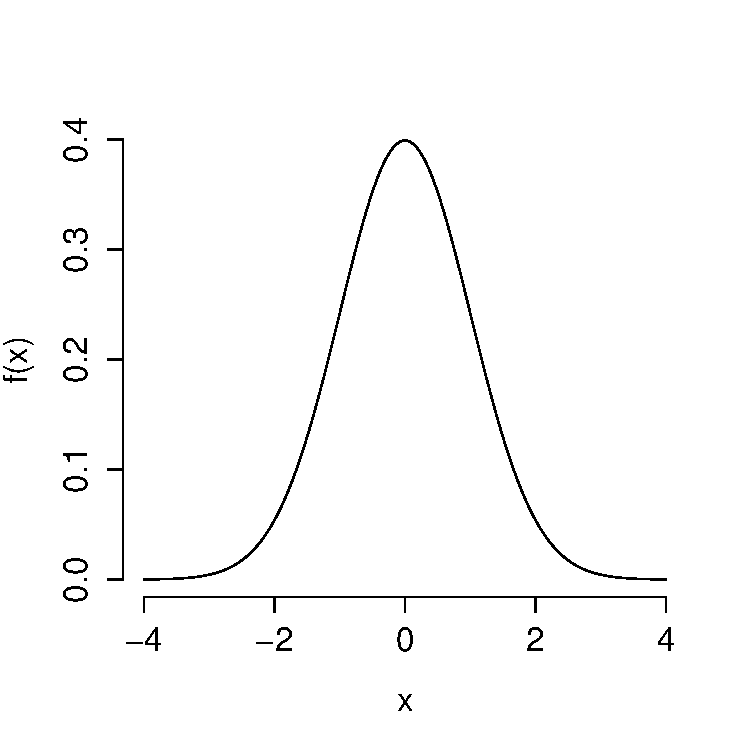
\includegraphics[scale = 0.28]{./images/std_normal_PDF}
  &  
  \includegraphics[scale = 0.28]{./images/std_normal_CDF}
\end{tabular}
\caption{Standard Normal PDF (left) and CDF (Right)}
\end{figure}
\begin{itemize}
  \item Notation: $X \sim N(0,1)$
  \item Symmetric, Bell-shaped, $E[X]=0$, $Var[X]=1$
  \item Support Set $= (-\infty,\infty)$
\end{itemize}
\end{frame}

%%%%%%%%%%%%%%%%%%%%%%%%%%%%%%%%%%%%%%%%
\begin{frame}
  \frametitle{Standard Normal Random Variable: $N(0,1)$}
\begin{figure}[h]
  \centering
  \begin{tabular}{cc}
  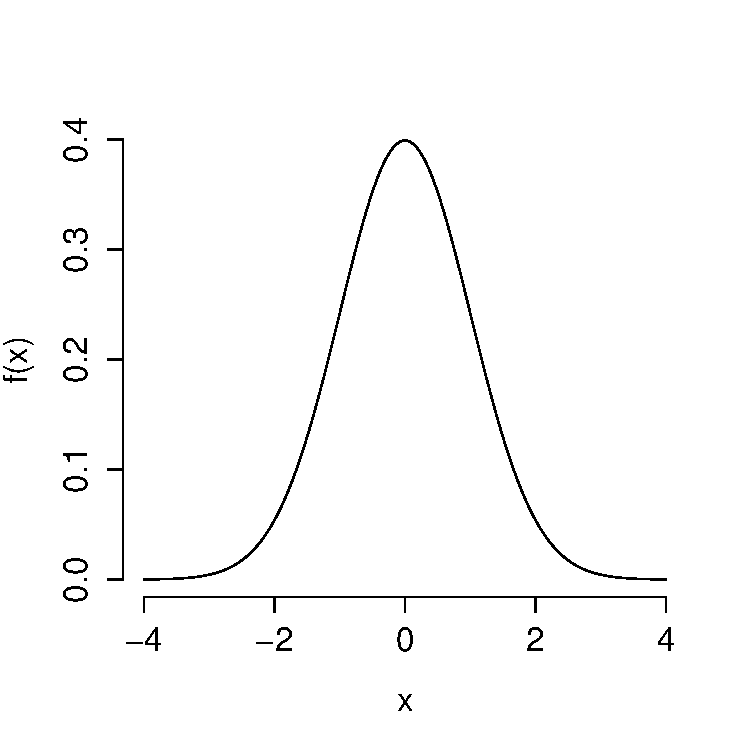
\includegraphics[scale = 0.3]{./images/std_normal_PDF}
  &  
  \includegraphics[scale = 0.3]{./images/std_normal_CDF}
\end{tabular}
\end{figure}
\begin{itemize}
  \item There is no closed-form expression for the $N(0,1)$ CDF.
  \item For Econ 103, don't need to know formula for $N(0,1)$ PDF.
  \item You \emph{do need} to know the R commands\dots
\end{itemize}
\end{frame}
%%%%%%%%%%%%%%%%%%%%%%%%%%%%%%%%%%%%%%%%
\begin{frame}
  \frametitle{R Commands for the Standard Normal RV}
  \begin{block}{\texttt{dnorm} -- \small Standard Normal PDF}
    \begin{itemize}
      \item Mnemonic: \texttt{d} $=$ density, \texttt{norm} $=$ normal
      \item Example: \texttt{dnorm(0)} gives height of $N(0,1)$ PDF at zero.
    \end{itemize}
  \end{block}
  \pause
  \begin{block}{\texttt{pnorm} -- \small Standard Normal CDF}
    \begin{itemize}
      \item Mnemonic: \texttt{p} $=$ probability, \texttt{norm} $=$ normal
      \item Example: $\texttt{pnorm(1)} = P(X\leq 1)$ if $X\sim N(0,1)$.
    \end{itemize}
  \end{block}
  \pause
  \begin{block}{\texttt{rnorm} -- \small Simulate Standard Normal Draws}
    \begin{itemize}
      \item Mnemonic: \texttt{r} $=$ random, \texttt{norm} $=$ normal. 
      \item Example: \texttt{rnorm(10)} makes ten iid $N(0,1)$ draws.
    \end{itemize}
  \end{block}
\end{frame}
%%%%%%%%%%%%%%%%%%%%%%%%%%%%%%%%%%%%%%%%
\begin{frame}
  \frametitle{$\Phi(x_0)$ Denotes the $N(0,1)$ CDF}
  You will sometimes encounter the notation $\Phi(x_0)$.
  It means the same thing as $\texttt{pnorm}(x_0)$ but it's not an R command. 
\end{frame}
%%%%%%%%%%%%%%%%%%%%%%%%%%%%%%%%%%%%%%%%
\begin{frame}
  \frametitle{The $N(\mu, \sigma^2)$ Random Variable}
  \begin{block}{Idea}
   Take a linear function of the $N(0,1)$ RV.
  \end{block}
  \begin{block}{Formal Definition}
    \alert{$N(\mu, \sigma^2) \equiv \mu + \sigma X$} where $X \sim N(0,1)$ and $\mu, \sigma$ are constants.
  \end{block}
  \begin{block}{Properties of $N(\mu, \sigma^2)$ RV}
    \begin{itemize}
      \item Parameters: Expected Value $= \mu$, Variance $= \sigma^2$
      \item Symmetric and bell-shaped. 
      \item Support Set $=(-\infty,\infty)$
      \item $N(0,1)$ is the special case where $\mu=0$ and $\sigma^2 = 1$. 
    \end{itemize}
  \end{block}
\end{frame}
%%%%%%%%%%%%%%%%%%%%%%%%%%%%%%%%%%%%%%%%
\begin{frame}
  \frametitle{Expected Value: $\mu$ \emph{shifts} PDF}

\begin{figure}
\includegraphics[scale = 0.45]{./images/normal_means}
\caption{\textcolor{blue}{Blue $\mu = -1$},
Black $\mu = 0$,
\textcolor{red}{Red $\mu = 1$}}
\end{figure}
\end{frame}

%%%%%%%%%%%%%%%%%%%%%%%%%%%%%%%%%%%%%%%%


\begin{frame}
  \frametitle{Standard Deviation: $\sigma$ \emph{scales} PDF}

\begin{figure}
\includegraphics[scale = 0.44]{./images/normal_std_devs}
\caption{\textcolor{blue}{Blue $\sigma^2 = 4$},
Black $\sigma^2=1$,
\textcolor{red}{Red $\sigma^2= 1/4$}}
\end{figure}
\end{frame}

%%%%%%%%%%%%%%%%%%%%%%%%%%%%%%%%%%%%%%%%


\begin{frame}
\frametitle{Linear Function of Normal RV is a Normal RV}


Suppose that $X \sim N(\mu, \sigma^2)$. Then if $a$ and $b$ constants,
$$\boxed{a + bX \sim N(a + b\mu, b^2 \sigma^2)}$$

\begin{block}{Important}
	\begin{itemize}
    \item  For \emph{any} RV $X$, $E[a + bX] = a +bE[X]$ and $Var(a +bX) = b^2 Var(X)$.
		\item Key point: linear transformation of normal is still normal!
    \item Linear transformation of Binomial is \emph{not} Binomial!
	\end{itemize}
\end{block}

\end{frame}

%%%%%%%%%%%%%%%%%%%%%%%%%%%%%%%%%%%%%%%%
\begin{frame}
\frametitle{Example}
Suppose $X \sim N(\mu, \sigma^2)$ and let $Z = (X -\mu)/\sigma$. What is the distribution of $Z$?

\begin{enumerate}[(a)]
	\item $N(\mu, \sigma^2)$
	\item $N(\mu, \sigma)$
	\item $N(0, \sigma^2)$
	\item  $N(0, \sigma)$
	\item $N(0,1)$
\end{enumerate}
\end{frame}

%%%%%%%%%%%%%%%%%%%%%%%%%%%%%%%%%%%%%%%%
\begin{frame}
  \frametitle{Linear Combinations of \emph{Multiple Independent} Normals}
Let $X \sim N(\mu_x, \sigma^2_x)$ independent of $Y \sim N(\mu_y, \sigma^2_y)$. Then if $a,b,c$ are constants:

$$\boxed{aX + bY +c \sim N(a\mu_x + b\mu_y + c, a^2 \sigma_x^2 + b^2 \sigma_y^2)}$$



\begin{block}{Important}
	\begin{itemize}
		\item Result assumes independence
		\item Particular to Normal RV 
		\item Extends to more than two Normal RVs
	\end{itemize}
\end{block}

\end{frame}
%%%%%%%%%%%%%%%%%%%%%%%%%%%%%%%%%%%%%%%%
\begin{frame}
\frametitle{Suppose $X_1, X_2, \sim \mbox{iid } N(\mu, \sigma^2)$}

Let $\bar{X} = (X_1 + X_2)/2$. What is the distribution of $\bar{X}$?
\begin{enumerate}[(a)]
\item $N(\mu, \sigma^2/2)$
\item $N(0,1)$
\item $N(\mu, \sigma^2)$
\item $N(\mu, 2\sigma^2)$
\item $N(2\mu, 2\sigma^2)$
\end{enumerate}

\end{frame}

%%%%%%%%%%%%%%%%%%%%%%%%%%%%%%%%%%%%%%%%
\begin{frame}
\frametitle{Where does the Empirical Rule come from?}

\begin{block}{Empirical Rule}
Approximately 68\% of observations within $\mu\pm \sigma$\\
Approximately 95\% of observations within $\mu\pm 2 \sigma$\\
Nearly all observations within $\mu\pm 3 \sigma$
\end{block}
\end{frame}

%%%%%%%%%%%%%%%%%%%%%%%%%%%%%%%%%%%%%%%%

\begin{frame}
\frametitle{\texttt{pnorm(1)}$\approx 0.84$}

\begin{figure}
\includegraphics[scale = 0.5]{./images/middle68_1}
\end{figure}
\end{frame}
%%%%%%%%%%%%%%%%%%%%%%%%%%%%%%%%%%%%%%%%
\begin{frame}
\frametitle{\texttt{pnorm(1) - pnorm(-1)}$\approx 0.84 - 0.16$}
\begin{figure}
\includegraphics[scale = 0.5]{./images/middle68_2}
\end{figure}
\end{frame}
%%%%%%%%%%%%%%%%%%%%%%%%%%%%%%%%%%%%%%%%
\begin{frame}
\frametitle{\texttt{pnorm(1) - pnorm(-1)}$\approx 0.68$}
\begin{figure}
\includegraphics[scale = 0.5]{./images/middle68_3}
\end{figure}
\end{frame}
%%%%%%%%%%%%%%%%%%%%%%%%%%%%%%%%%%%%%%%%

\begin{frame}
\frametitle{Middle 68\% of $N(0,1) \Rightarrow$ approx.\ $(-1,1)$}
\begin{figure}
\includegraphics[scale = 0.5]{./images/normal_middle68}
\end{figure}
\end{frame}

%%%%%%%%%%%%%%%%%%%%%%%%%%%%%%%%%%%%%%%%
\begin{frame}
\frametitle{Suppose $X \sim N(0,1)$}
\begin{eqnarray*}
	P(-1 \leq X \leq 1) &=& \mbox{\texttt{pnorm(1) - pnorm(-1)}}\\
		&\approx& 0.683
\end{eqnarray*}
\begin{eqnarray*}
	P(-2 \leq X \leq 2) &=& \mbox{\texttt{pnorm(2) - pnorm(-2)}}\\
		&\approx& 0.954
\end{eqnarray*}
\begin{eqnarray*}
	P(-3 \leq X \leq 3) &=& \mbox{\texttt{pnorm(3) - pnorm(-3)}}\\
		&\approx& 0.997
\end{eqnarray*}

\end{frame}
%%%%%%%%%%%%%%%%%%%%%%%%%%%%%%%%%%%%%%%%
\begin{frame}
\frametitle{What if $X \sim N(\mu, \sigma^2)$?}
\begin{eqnarray*}
	P(X \leq a) &=& \pause P(X - \mu \leq a - \mu)\\\\
		&=& \pause P\left( \frac{X-\mu}{\sigma} \leq \frac{a - \mu}{\sigma} \right)\\\\
		&=&\pause  P\left(Z \leq  \frac{a - \mu}{\sigma}\right)
\end{eqnarray*}
Where $Z$ is a standard normal random variable, i.e.\ $N(0,1)$.
\end{frame}


%%%%%%%%%%%%%%%%%%%%%%%%%%%%%%%%%%%%%%%%
\begin{frame}
Which of these equals $P\left(Z \leq (a-\mu)/\sigma\right)$ if $Z\sim N(0,1)$?
	\begin{enumerate}[(a)]
    \item $\texttt{pnorm(a)}$
    \item $1 - \texttt{pnorm(a)}$
    \item $\texttt{pnorm(a)}/\sigma - \mu$
    \item $\texttt{pnorm}\left(\frac{a - \mu}{\sigma}  \right)$
		\item None of the above.
	\end{enumerate}
\end{frame}

%%%%%%%%%%%%%%%%%%%%%%%%%%%%%%%%%%%%%%%%
\begin{frame}
  \frametitle{Probability \emph{Above} a Threshold: $X \sim N(\mu, \sigma^2)$}
\begin{eqnarray*}
	P(X \geq b) &=&1 - P(X\leq b) =1 - P\left( \frac{X-\mu}{\sigma} \leq \frac{b-\mu}{\sigma} \right) \\ \\
	&=& 1 - P\left( Z \leq \frac{b-\mu}{\sigma} \right) \\
	&=& 1 -\mbox{\texttt{pnorm}}((b-\mu)/\sigma)
\end{eqnarray*}
Where $Z$ is a standard normal random variable.
\end{frame}
%%%%%%%%%%%%%%%%%%%%%%%%%%%%%%%%%%%%%%%%
\begin{frame}
\frametitle{Probability of an Interval: $X \sim N(\mu, \sigma^2)$}


\begin{eqnarray*}
	P(a \leq X \leq b) &=&  P\left( \frac{a - \mu}{\sigma} \leq \frac{X - \mu}{\sigma} \leq \frac{b-\mu}{\sigma} \right)\\ \\ 
	&=& P\left( \frac{a - \mu}{\sigma} \leq Z \leq \frac{b-\mu}{\sigma} \right)\\ \\ 
	&=&\ \mbox{\texttt{pnorm}}((b-\mu)/\sigma) -  \mbox{\texttt{pnorm}}((a-\mu)/\sigma)
\end{eqnarray*}
Where $Z$ is a standard normal random variable.
\end{frame}
%%%%%%%%%%%%%%%%%%%%%%%%%%%%%%%%%%%%%%%%
\begin{frame}
\frametitle{Suppose $X \sim N(\mu, \sigma^2)$}
What is $P(\mu - \sigma \leq X \leq \mu + \sigma)$?

\pause
\begin{eqnarray*}
P(\mu - \sigma \leq X \leq \mu + \sigma) &=& P\left( -1 \leq \frac{X-\mu}{\sigma} \leq 1\right)\\ \\
	&=& P\left( -1 \leq Z \leq 1\right)\\
	&=& \mbox{\texttt{pnorm(1)}} -  \mbox{\texttt{pnorm(-1)}}\\
	&\approx& 0.68
\end{eqnarray*}
\end{frame}

%%%%%%%%%%%%%%%%%%%%%%%%%%%%%%%%%%%%%%%%

\begin{frame}
\frametitle{Percentiles/Quantiles for Continuous RVs}
\begin{block}{Quantile Function $Q(p)$ is the inverse of CDF $F(x_0)$}
Plug in a probability $p$, get out the value of $x_0$ such that $F(x_0)=p$
\end{block}
$$Q(p) = F^{-1}(p)$$

In other words:
	$$Q(p) = \mbox{the value of } x_0 \mbox{ such that } \int_{-\infty}^{x_0} f(x) \; dx = p$$
	
\begin{alertblock}{Inverse exists as long as $F(x_0)$ is \emph{strictly increasing}.} \end{alertblock}	
	
\end{frame}
%%%%%%%%%%%%%%%%%%%%%%%%%%%%%%%%%%%%%%%%
\begin{frame}
\frametitle{Example: Median}
The median of a continuous random variable is $Q(0.5)$, i.e.\ the value of $x_0$ such that 
	$$\int_{-\infty}^{x_0} f(x)\; dx = 1/2$$
\end{frame}
%%%%%%%%%%%%%%%%%%%%%%%%%%%%%%%%%%%%%%%%
\begin{frame}
\frametitle{What is the median of a standard normal RV?}
\pause
By symmetry, $Q(0.5) = 0$. R command: \texttt{qnorm()}
\begin{center}
\includegraphics[scale = 0.47]{./images/normal_median}
\end{center}
\end{frame}
%%%%%%%%%%%%%%%%%%%%%%%%%%%%%%%%%%%%%%%%
\begin{frame}
\frametitle{90th Percentile of a Standard Normal}
\texttt{qnorm(0.9)}$\approx 1.28$
\begin{center}
\includegraphics[scale = 0.47]{./images/normal90}
\end{center}
\end{frame}
%%%%%%%%%%%%%%%%%%%%%%%%%%%%%%%%%%%%%%%%

\begin{frame}
\frametitle{Using Quantile Function to find Symmetric Intervals}
Suppose $X$ is a standard normal RV. What is the value of $c$ such that $P(-c \leq X\leq c ) = 0.5$?
\begin{center}
\includegraphics[scale = 0.45]{./images/tail1}
\end{center}
\end{frame}

%%%%%%%%%%%%%%%%%%%%%%%%%%%%%%%%%%%%%%%%
\begin{frame}
\frametitle{\texttt{qnorm(0.75)}$\approx 0.67$}
Suppose $X$ is a standard normal RV. What is the value of $c$ such that $P(-c \leq X\leq c ) = 0.5$?
\begin{center}
\includegraphics[scale = 0.5]{./images/tail2}
\end{center}
\end{frame}

%%%%%%%%%%%%%%%%%%%%%%%%%%%%%%%%%%%%%%%%
\begin{frame}
\frametitle{\texttt{qnorm(0.75)}$\approx 0.67$}
Suppose $X$ is a standard normal RV. What is the value of $c$ such that $P(-c \leq X\leq c ) = 0.5$?
\begin{center}
\includegraphics[scale = 0.55]{./images/tail3}
\end{center}
\end{frame}

%%%%%%%%%%%%%%%%%%%%%%%%%%%%%%%%%%%%%%%%

\begin{frame}
\frametitle{\texttt{pnorm(0.67)-pnorm(-0.67)}$\approx$?}
Suppose $X$ is a standard normal RV. What is the value of $c$ such that $P(-c \leq X\leq c ) = 0.5$?
\begin{center}
\includegraphics[scale = 0.55]{./images/tail4}
\end{center}
\end{frame}

%%%%%%%%%%%%%%%%%%%%%%%%%%%%%%%%%%%%%%%%


\begin{frame}
\frametitle{\texttt{pnorm(0.67)-pnorm(-0.67)}$\approx 0.5$}
Suppose $X$ is a standard normal RV. What is the value of $c$ such that $P(-c \leq X\leq c ) = 0.5$?
\begin{center}
\includegraphics[scale = 0.55]{./images/tail5}
\end{center}
\end{frame}
%%%%%%%%%%%%%%%%%%%%%%%%%%%%%%%%%%%%%%%%
\begin{frame}
\frametitle{95\% Central Interval for Standard Normal}

Suppose $X$ is a standard normal random variable. What value of $c$ ensures that $P(-c \leq X \leq c) \approx \alert{0.95}$?

\end{frame}


%%%%%%%%%%%%%%%%%%%%%%%%%%%%%%%%%%%%%%%%

\begin{frame}
  \frametitle{R Commands for \emph{Arbitrary} Normal RVs}
Let $X \sim N(\mu, \sigma^2)$ . Then we can use R to evaluate the CDF and Quantile function of $X$ as follows:
\vspace{1em}
\begin{table}
\centering
\fbox{\begin{tabular}{ll}
CDF $F(x)$&\texttt{pnorm(x, mean = $\mu$,  sd = $\sigma$)}\\
Quantile Function $Q(p)$ & \texttt{qnorm(p, mean = $\mu$,  sd = $\sigma$)}\\
\end{tabular}}
\end{table}
\vspace{1em}
\alert{Notice that this means you don't have to transform $X$ to a standard normal in order to find areas under its pdf using R.}
\end{frame}
%%%%%%%%%%%%%%%%%%%%%%%%%%%%%%%%%%%%%%%%
\begin{frame}
\frametitle{Example: $X \sim N(0,16)$}

One Way:
			\begin{eqnarray*}
				P(X \geq 10) &=&  1 - P(X \leq 10) = 1 - P(X /4\leq 10/4)\\
				&=& 1 - P(Z\leq 2.5) =   1 - \Phi(2.5) =  1 - \mbox{\texttt{pnorm(2.5)}}\\ 
				&\approx& 0.006
			\end{eqnarray*}
\pause
An Easier Way:
	\begin{eqnarray*}
	P(X \geq 10) &=& 1 - P(X \leq 10)\\ 
	&=&  1 - \texttt{pnorm(10, mean = 0, sd = 4)} \\ 
	&\approx& 0.006
	\end{eqnarray*}
\end{frame}

%%%%%%%%%%%%%%%%%%%%%%%%%%%%%%%%%%%%%%%%
\begin{frame}
\frametitle{What's Next?}
\begin{itemize}[<+-|alert@+>]
	\item We've discussed a lot about normal random variables
	\item Hopefully, you're starting to feel more confident about how to use them
	\item And maybe you're even starting to wonder if there's something more to the normal random variable
	\item What if...?
\end{itemize}
\end{frame}

\section{Chi Squared Distribution}
%%%%%%%%%%%%%%%%%%%%%%%%%%%%%%%%%%%%%%%%
\begin{frame}
\begin{figure}
\includegraphics[scale = 0.45]{./images/chisq_etsy1}
\caption{PDF for $\chi^2$-Distribution}
\end{figure}
\end{frame}

%%%%%%%%%%%%%%%%%%%%%%%%%%%%%%%%%%%%%%%
\begin{frame}
\begin{figure}
\includegraphics[scale = 0.45]{./images/chisq_etsy_witch}
\caption{$\chi^2$ PDF -- Halloween Edition}
\end{figure}
\end{frame}

%%%%%%%%%%%%%%%%%%%%%%%%%%%%%%%%%%%%%%%%
\begin{frame}
\begin{figure}
\includegraphics[scale = 0.45]{./images/chisq_etsy2}
\end{figure}
\end{frame}
%%%%%%%%%%%%%%%%%%%%%%%%%%%%%%%%%%%%%%%%
\begin{frame}
\frametitle{$\chi^2$ Random Variable}
Let $X_1, \hdots, X_\nu \sim \mbox{iid } N(0,1)$. Then,
	$$\left(X_1^2 + \hdots + X_\nu^2  \right)\sim \chi^2(\nu)$$
	where the parameter $\nu$ is the \emph{degrees of freedom}
	
	\vspace{1em}
	\pause
	\alert{Support = $(0, \infty)$}\\
	\vspace{1em}
\end{frame}




%%%%%%%%%%%%%%%%%%%%%%%%%%%%%%%%%%%%%%%%

\begin{frame}
\frametitle{$\chi^2$ PDFs}

\begin{figure}
\includegraphics[scale = 0.58]{./images/chisq}
\end{figure}
\end{frame}

\section{t-Distribution}
%%%%%%%%%%%%%%%%%%%%%%%%%%%%%%%%%%%%%%%

\begin{frame}
\begin{figure}
\includegraphics[scale = 0.2]{./images/t_etsy1}
\caption{PDF for Student-t Distribution}
\end{figure}
\end{frame}

%%%%%%%%%%%%%%%%%%%%%%%%%%%%%%%%%%%%%%%%
\begin{frame}
\begin{figure}
\includegraphics[scale = 0.2]{./images/t_etsy2}
\end{figure}
\end{frame}

%%%%%%%%%%%%%%%%%%%%%%%%%%%%%%%%%%%%%%%%

\begin{frame}
\frametitle{Student-t Random Variable}
Let $X \sim N(0,1)$ independent of $Y \sim \chi^2(\nu)$. Then,
$$\frac{X}{\sqrt{Y/\nu}}\sim t(\nu)$$
where the parameter $\nu$ is the degrees of freedom.

\pause

\begin{itemize}
	\item Support = $(-\infty, \infty)$
	\item As $\nu \rightarrow \infty$, $t \rightarrow$ Standard Normal.
	\item Symmetric around zero, but mean and variance may not exist!
	\item Degrees of freedom $\nu$ control ``thickness of tails''
\end{itemize}
\vspace{1em}


\end{frame}

%%%%%%%%%%%%%%%%%%%%%%%%%%%%%%%%%%%%%%%%
\begin{frame}
\frametitle{Student-t PDFs}

\begin{figure}
\includegraphics[scale = 0.58]{./images/tpdf}
\end{figure}
\end{frame}

\section{F Distribution}
%%%%%%%%%%%%%%%%%%%%%%%%%%%%%%%%%%%%%%%%
\begin{frame}
\frametitle{F Random Variable}
Suppose $X \sim \chi^2(\nu)$ independent of $Y \sim \chi^2(\omega)$. Then,
	$$\frac{X/\nu}{Y/\omega} \sim F(\nu, \omega)$$
where $\nu$ is the numerator degrees of freedom and $\omega$ is the denominator degrees of freedom.
\vspace{1em}


\alert{Support = $(0, \infty)$}\\

\end{frame}




%%%%%%%%%%%%%%%%%%%%%%%%%%%%%%%%%%%%%%%%
\begin{frame}
\frametitle{F PDFs}

\begin{figure}
\includegraphics[scale = 0.58]{./images/Fdist}
\end{figure}
\end{frame}

\section{R Commands}
%%%%%%%%%%%%%%%%%%%%%%%%%%%%%%%%%%%%%%%%

\begin{frame}
\frametitle{R Commands -- CDFs and Quantile Functions}
$F(x) = P(X\leq x)$ is the CDF, $Q(p) = F^{-1}(p)$ the Quantile Function
\footnotesize
\begin{table}
\begin{tabular}{l|ll}
&$F(x)$&$Q(p)$\\
\hline
$N(\mu,\sigma^2)$ &\texttt{pnorm(x, mean = $\mu$,  sd = $\sigma$)}&\texttt{qnorm(p, mean = $\mu$,  sd = $\sigma$)}\\
$\chi^2(\nu)$&\texttt{pchisq(x, df = $\nu$)}&\texttt{qchisq(p, df = $\nu$)}\\
$t(\nu)$&\texttt{pt(x, df = $\nu$)}&\texttt{qt(p, df = $\nu$)}\\
$F(\nu,\omega)$&\texttt{pf(x, df1 = $\nu$, df2 = $\omega$)}&\texttt{qf(p, df1 = $\nu$, df2 = $\omega$)}
\end{tabular}
\end{table}
\vspace{1em}
\normalsize
\alert{Mnemonic: ``p'' is for Probability, ``q'' is for Quantile.}

\end{frame}
%%%%%%%%%%%%%%%%%%%%%%%%%%%%%%%%%%%%%%%%
\begin{frame}
\frametitle{R Commands -- PDFs and Random Draws}
\footnotesize
\begin{table}
\begin{tabular}{l|ll}
&$f(x)$&Make \texttt{n} iid Random Draws\\
\hline
$N(\mu,\sigma^2)$ &\texttt{dnorm(x, mean = $\mu$,  sd = $\sigma$)}&\texttt{rnorm(n, mean = $\mu$,  sd = $\sigma$)}\\
$\chi^2(\nu)$&\texttt{dchisq(x, df = $\nu$)}&\texttt{rchisq(n, df = $\nu$)}\\
$t(\nu)$&\texttt{dt(x, df = $\nu$)}&\texttt{rt(n, df = $\nu$)}\\
$F(\nu,\omega)$&\texttt{df(x, df1 = $\nu$, df2 = $\omega$)}&\texttt{rf(n, df1 = $\nu$, df2 = $\omega$)}
\end{tabular}
\end{table}
\vspace{1em}
\normalsize
\alert{Mnemonic: ``d'' is for Density, ``r'' is for Random.}

\end{frame}

\section{Practice}
%%%%%%%%%%%%%%%%%%%%%%%%%%%%%%%%%%%%%%%%


\begin{frame}
\frametitle{Example: $X_1, X_2, X_3 \sim \mbox{iid } N(0, 1)$}
\begin{block}{What is the distribution of $Y_1 = X_1^2 + X_2^2$?}\pause
Sum of squares of two indep.\ std.\ normals $\Rightarrow \alert{Y_1 \sim \chi^2(2)}$
\end{block}
\pause
\begin{block}{What is the distribution of $Y_2 = (Y_1/2)/(X_3^2)$?}
\pause
$Y_1 \sim \chi^2(2)$ and $X_3^2 \sim \chi^2(1)$\\
\pause
\vspace{1em}
Hence $Y_2 =$ ratio of two indep.\ $\chi^2$ RVs, each divided by its degrees of freedom $\Rightarrow \alert{Y_2 \sim F(2,1)}$
\end{block}
\pause
\begin{block}{What is the distribution of $Z = X_3/\sqrt{Y_1/2}$?}
\pause
Ratio of standard normal and square root of independent $\chi^2$ RV divided by its degrees of freedom $\Rightarrow \alert{Z \sim t(2)}$
\end{block}
\end{frame}
%%%%%%%%%%%%%%%%%%%%%%%%%%%%%%%%%%%%%%%%
\begin{frame}
\frametitle{Suppose $X_1, X_2, \sim \mbox{iid } N(\mu, \sigma^2)$ }
Let $Y = \left( X_1 - \mu\right)^2 + \left( X_2 - \mu\right)^2$. What is the distribution of $Y/\sigma^2$?

\begin{enumerate}[(a)]
	\item $F(2,1)$
	\item $\chi^2(2)$
	\item $t(2)$
	\item $N(\mu, \sigma)$
	\item None of the above
\end{enumerate}

\end{frame}
%%%%%%%%%%%%%%%%%%%%%%%%%%%%%%%%%%%%%%%%
\begin{frame}
\frametitle{$Y_1 \sim \chi^2(2),\;\;\;\; Y_2 \sim F(2,1),\;\;\;\; Z \sim t(2)$}
\begin{block}{What is the median of $Y_1$?}
\pause
\texttt{qchisq(0.5, df = 2)}$\approx 1.4$
\end{block}
\pause
\begin{block}{What is $P(Y_2 \leq 5)$?}
\pause
\texttt{pf(5, df1 = 2, df2 = 1)}$\approx 0.7$
\end{block}
\pause
\begin{block}{What value of $c$ gives $P(-c\leq Z \leq c) = 0.5$?}
Use Symmetry (like normal) \\
$c=$\texttt{qt(0.75, df = 2)}$\approx 0.8$ 
\pause
\\or equivalently $-c =$\texttt{qt(0.25, df = 2)}$\approx -0.8$
\end{block}

\end{frame}

%%%%%%%%%%%%%%%%%%%%%%%%%%%%%%%%%%%%%%%%

\end{document}